\chapter[Software de simulação]{Software de simulação no desenvolvimento de enxames}\label{cap:sim}
A simulação computacional representa veículos e ambientes para examinar decisões de navegação antes da operação física. No caso de um enxame, permite observar como as trajetórias individuais se combinam: onde os agentes se aproximam, como atravessam uma passagem e como alteram o movimento diante de um obstáculo. Essas situações relacionam os algoritmos de coordenação ao comportamento do grupo.

\section{Trajetórias, conflitos e separação entre agentes}
Um destino alcançável por um drone pode produzir conflitos quando vários veículos tentam alcançá-lo ao mesmo tempo. O simulador permite representar esses encontros e examinar as respostas do sistema. Trajetórias, posições e informações de percepção ajudam a distinguir o caminho pretendido, o movimento calculado e os obstáculos considerados pelo planejador.

A visualização também permite identificar situações que precisam de análise nos registros. Duas trajetórias que se cruzam na imagem, por exemplo, não demonstram uma colisão: os veículos podem passar pelo mesmo ponto em instantes diferentes ou em altitudes distintas. Para avaliar a separação, é necessário relacionar as posições ao tempo e às dimensões dos veículos. Assim, as figuras ajudam a interpretar o movimento, enquanto os registros sustentam sua avaliação quantitativa.

\section{Exemplos de coordenação em ambientes simulados}
\subsection{Navegação, formação e obstáculos móveis}
Zhou et al.~\cite{wildpaper} disponibilizaram um ambiente denominado \emph{swarm playground}, com exemplos de navegação de 40 drones, voo em formação, troca de posições e desvio de obstáculos móveis. A Figura~\ref{fig:swarm-playground} reúne quatro dessas situações. O estudo também incluiu voos físicos; os painéis selecionados são exclusivamente simulações.

No painel A, os percursos individuais atravessam um campo de obstáculos. No painel B, o grupo mantém uma organização geométrica. Os painéis C e F acrescentam conflitos entre trajetórias e mudanças no ambiente. Esses exemplos mostram como o software permite examinar diferentes exigências de coordenação antes da integração com as aeronaves.

\begin{figure}[htbp]
\centering
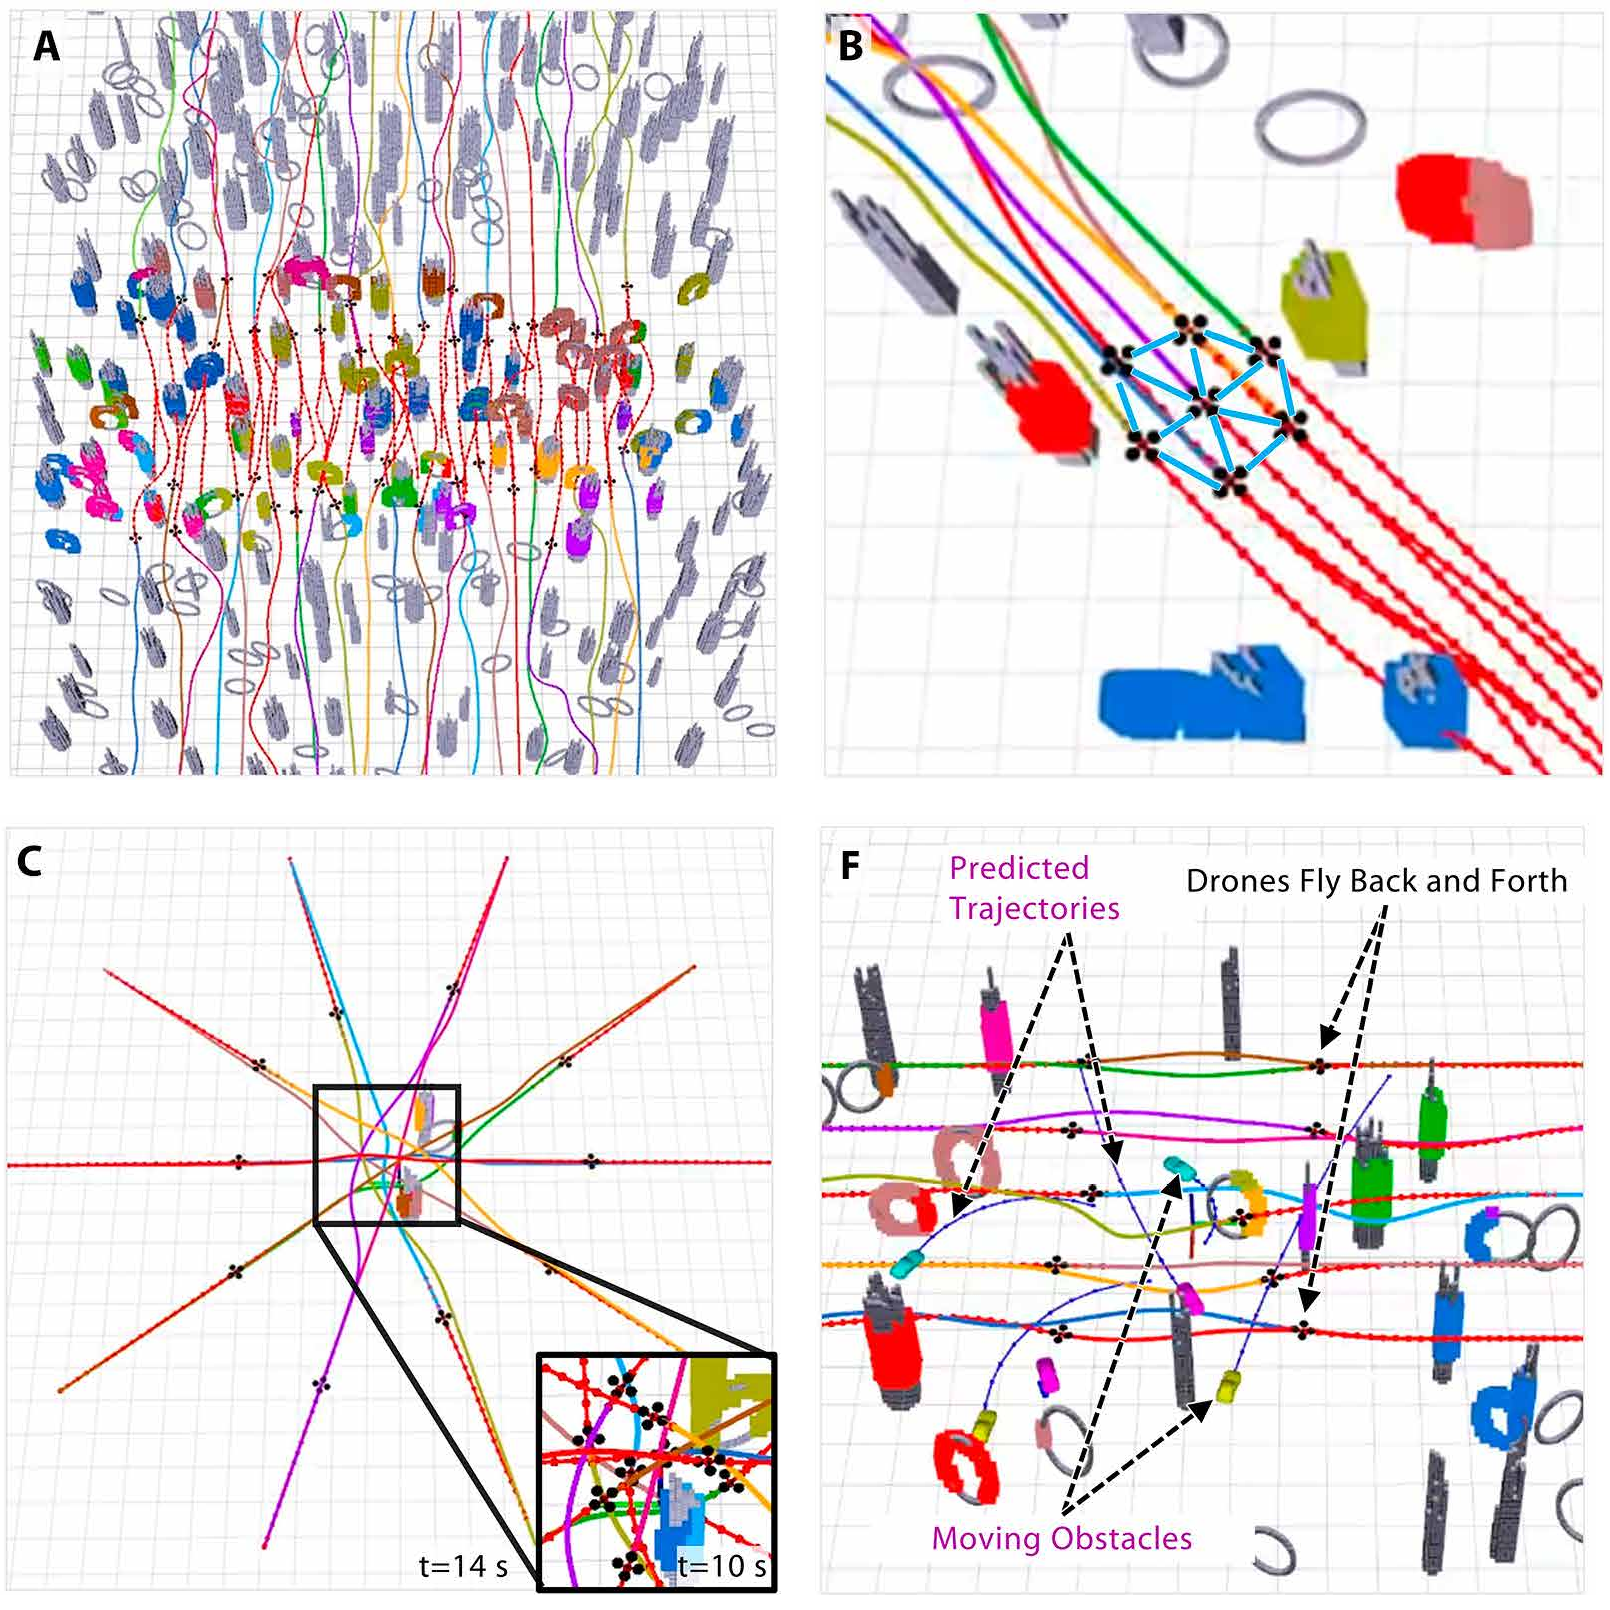
\includegraphics[width=0.91\textwidth]{swarm-playground-comportamentos.png}
\caption[Comportamentos de enxame no swarm playground]{Simulações no \emph{swarm playground}: (A) navegação de 40 drones; (B) formação; (C) troca de posições em um círculo; (F) desvio de obstáculos móveis. As linhas contínuas coloridas representam trajetórias anteriores; as vermelhas com marcadores, trajetórias planejadas; os símbolos pretos, drones; os objetos cinzentos, obstáculos ainda não percebidos; e os coloridos, obstáculos percebidos. Em B, os segmentos cianos indicam a formação. Seleção e reorganização dos painéis A, B, C e F da Figura~8 de Zhou et al.~\cite{wildpaper}, preservando suas letras e separando-os por faixas brancas.}
\label{fig:swarm-playground}
\end{figure}

\subsection{Coordenação em ambientes com passagens}
O projeto \emph{Swarm Simulation}, descrito por Jiahao em 2018, apresenta demonstrações em Gazebo e AirSim~\cite{jiahaoswarm}. A Figura~\ref{fig:jiahao-enxame} mostra robôs terrestres no Gazebo. Embora não represente voo, o exemplo permite discutir um problema comum aos sistemas com vários agentes: coordenar deslocamentos em um espaço compartilhado.

\begin{figure}[htbp]
\centering
\begin{minipage}[c]{0.55\textwidth}
\centering
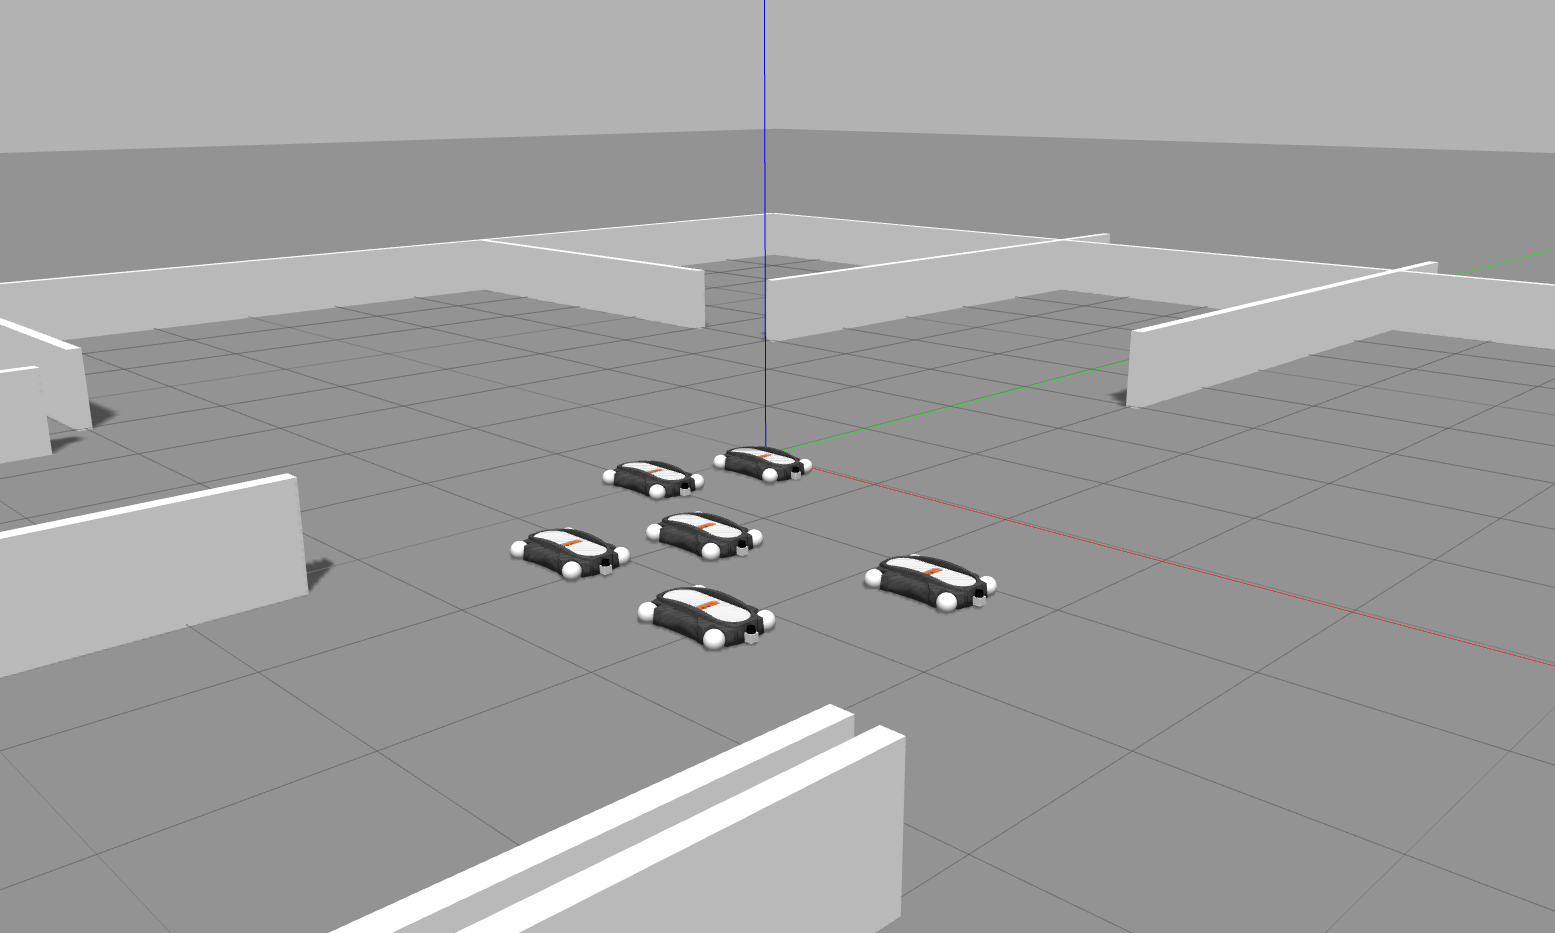
\includegraphics[width=\linewidth]{jiahao-enxame-gazebo.png}
\end{minipage}\hfill
\begin{minipage}[c]{0.42\textwidth}
\centering
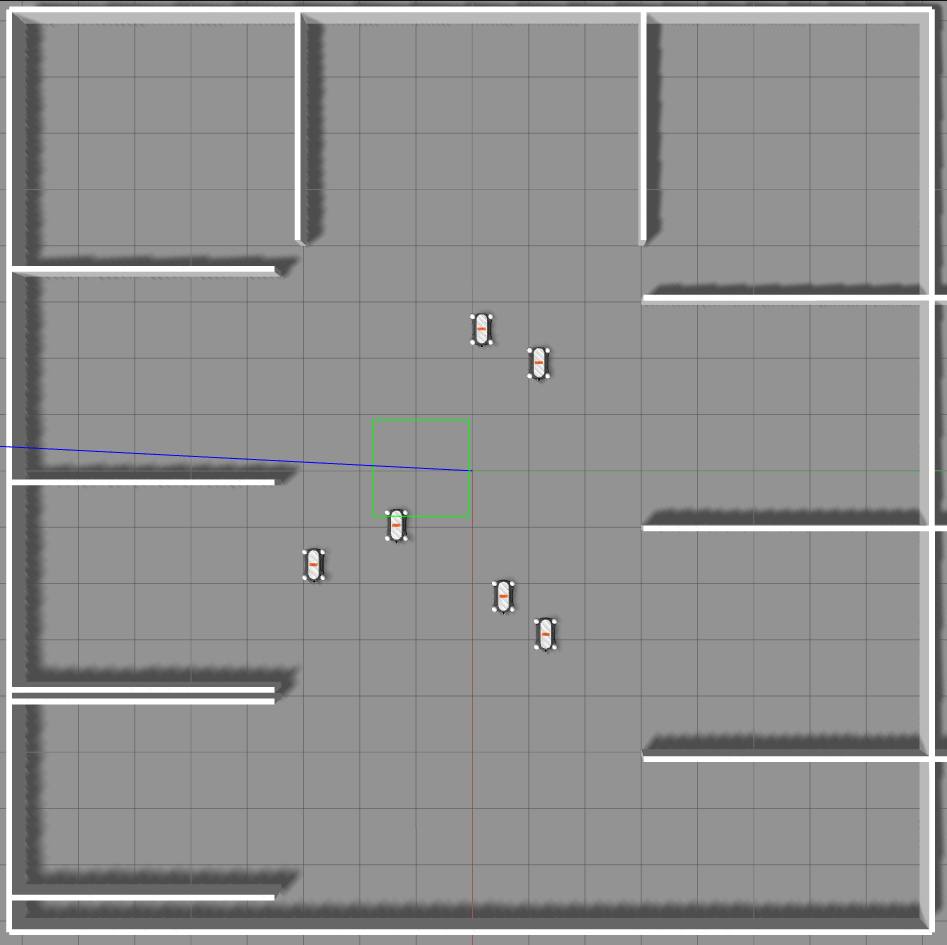
\includegraphics[width=\linewidth]{jiahao-enxame-mapa.png}
\end{minipage}
\caption[Grupo de robôs em ambiente Gazebo com passagens]{Exemplo do projeto \emph{Swarm Simulation}: à esquerda, bases KUKA YouBot em um cenário Gazebo; à direita, vista superior do ambiente com os robôs e uma região delimitada em verde. As paredes definem salas e passagens. As capturas mostram a configuração espacial, sem registrar a evolução temporal do movimento. Reprodução de imagens disponibilizadas por Jiahao~\cite{jiahaoswarm}.}
\label{fig:jiahao-enxame}
\end{figure}

O autor relata bloqueios quando vários robôs recebem o mesmo ponto de destino. A alternativa descrita foi distribuir destinos dentro de uma região, em vez de concentrá-los em uma única posição~\cite{jiahaoswarm}. O caso ilustra como a simulação pode revelar um conflito na definição da tarefa, antes de atribuí-lo ao controle do veículo. As demonstrações em vídeo estão disponíveis na \href{https://www.jiahaoz.com/swarm-simulation}{página do projeto}.

\FloatBarrier
\section{Ferramentas de simulação e integração}
As situações ilustradas exigem representações diferentes conforme o aspecto investigado. Para estudar regras de formação, pode ser suficiente representar posições, velocidades e vizinhanças. Para examinar navegação com câmeras ou respostas do controlador, são necessários modelos de sensores ou da dinâmica da aeronave. A Tabela~\ref{tab:simuladores} relaciona ferramentas a essas funções.

\subsection{Análise da coordenação}
O SwarmLab é um simulador desenvolvido em MATLAB para estudar drones individuais e enxames. Disponibiliza modelos de massa pontual e de quadricóptero, regras de interação e recursos de visualização e análise~\cite{swarmlab,swarmrepo}. Permite examinar a relação entre os parâmetros de coordenação e as trajetórias do grupo. Um modelo de massa pontual, entretanto, não representa diretamente atitude, motores ou dimensões da estrutura. Os exemplos de trajetórias do Capítulo~\ref{cap:casos} complementam essa aplicação.

\subsection{Integração com o software de voo}
Em uma configuração \emph{software-in-the-loop} (SITL), a pilha de voo é executada no computador e conectada a um modelo de veículo. Isso permite examinar comandos, estados e modos de operação antes de conectar uma controladora física. PX4 e ArduPilot documentam esse tipo de execução~\cite{px4sim,ardusitl}.

O Gazebo representa a dinâmica, sensores e objetos do ambiente~\cite{gazebo}. Na integração com PX4, calcula o movimento e fornece informações à pilha de voo, que produz os comandos de controle~\cite{px4gazebo}. Essa organização permite investigar a cadeia entre percepção, planejamento e resposta da aeronave simulada. A presença de um obstáculo na cena só influencia a percepção quando os sensores e o processamento utilizados o representam.

\subsection{Supervisão de missões e integração com a plataforma}
O QGroundControl fornece recursos de configuração, planejamento e acompanhamento de missões~\cite{qgc}. Durante a simulação, pode apresentar estados da pilha de voo e instruções enviadas ao veículo. Sua função é a de estação de solo; o cálculo da dinâmica cabe ao simulador conectado ao sistema.

O Crazyswarm2 documenta recursos de simulação no ecossistema Crazyflie e ROS~2~\cite{crazyswarm2}. Ferramentas vinculadas à plataforma permitem verificar componentes da aplicação e suas interfaces antes da conexão com as aeronaves. É necessário verificar quais interfaces e funções utilizadas na simulação também estão disponíveis nas aeronaves.

\begin{table}[htbp]
\centering\small
\caption{Ferramentas de apoio ao desenvolvimento e atividades descritas em suas documentações.}
\label{tab:simuladores}
\begin{tabularx}{\textwidth}{@{}>{\raggedright\arraybackslash}p{3cm}YY@{}}
\toprule
Ferramenta & Atividade apoiada & Aspecto a verificar \\
\midrule
SwarmLab & Examinar regras de interação e movimento coletivo & Modelo do agente e parâmetros da coordenação \\
Gazebo com PX4 & Examinar voo e navegação em ambiente simulado & Dinâmica, sensores e integração com a pilha de voo \\
ArduPilot SITL & Verificar operação e integração do software de voo & Modelo do veículo e interfaces da aplicação \\
QGroundControl & Configurar, planejar e acompanhar missões & Conexão com a pilha de voo e instruções da missão \\
Crazyswarm2 & Preparar aplicações no ecossistema Crazyflie & Correspondência entre recursos simulados e físicos \\
\bottomrule
\end{tabularx}
\end{table}

\section{Limites dos modelos e transferência para o voo real}\label{sec:limites-sim}
A simulação fornece evidência sobre o comportamento representado pelo modelo. Vibração, ruído dos sensores, interferência de rádio e consumo de energia só participam da avaliação quando são modelados. Mesmo nesses casos, a correspondência com o veículo depende de calibração ou de comparação com medições físicas.

Uma trajetória executada sem colisões no ambiente virtual não estabelece, por si só, a segurança do voo real. A contribuição da simulação está em examinar decisões de coordenação, identificar conflitos e verificar a integração de software. Os aspectos físicos que ela não representa precisam ser avaliados na plataforma escolhida.
